
\documentclass{package/notes}
\usepackage[english]{babel}
\usepackage{amssymb,amsmath,amsfonts}  %%% for maths
%%%%%%%%%%%%%%%%%%%%%%%%%%%%%%%%%%%%%
\usepackage{package/color-env}
\usepackage{lipsum}

\newcommand{\Z}{\mathbb{Z}}
\newcommand{\R}{\mathbb{R}}
\newcommand{\N}{\mathbb{N}}
\newcommand{\C}{\mathbb{C}}
\newcommand{\Q}{\mathbb{Q}}
\renewcommand\qedsymbol{$\blacksquare$}
%%%%%%%%%%%%%%%%%%%%%%%%%%%%%%%%%%%%%

\begin{document}

	\begin{titlepage} % Suppresses headers and footers on the title page
		
		\centering % Centre everything on the title page
		
		\scshape % Use small caps for all text on the title page
		
		\vspace*{\baselineskip} % White space at the top of the page
		
		%------------------------------------------------
		%	Title
		%------------------------------------------------
		
		\rule{\textwidth}{1.6pt}\vspace*{-\baselineskip}\vspace*{2pt} % Thick horizontal rule
		\rule{\textwidth}{0.4pt} % Thin horizontal rule
		
		\vspace{0.75\baselineskip} % Whitespace above the title
		
		{\huge MATH231 Discrete Structures Notes\\} % Title
		
		\vspace{0.75\baselineskip} % Whitespace below the title
		
		\rule{\textwidth}{0.4pt}\vspace*{-\baselineskip}\vspace{3.2pt} % Thin horizontal rule
		\rule{\textwidth}{1.6pt} % Thick horizontal rule
		
		\vspace{2\baselineskip} % Whitespace after the title block
		
		%------------------------------------------------
		%	Subtitle
		%------------------------------------------------
		
		
		
		\vspace*{3\baselineskip} % Whitespace under the subtitle
		
		
		
		\vspace{0.5\baselineskip} 
		
		
		
		\vspace{0.5\baselineskip} 
		
		
		
		\vfill 
		
		%------------------------------------------------
		% Author
		%------------------------------------------------
		
		
		\vspace{0.3\baselineskip} 
		
		
		{\large Edited by\\  Trevor Bushnell} 
		
	\end{titlepage}
	\tableofcontents
%\newpage
\chapter*{Introduction}

This document aims to highlight the important content of the MATH231 course in traditional notes format. These notes are completely open-source, which means anyone is allowed to use these notes for their own personal benefit without having to seek permission from myself. \newline

Due to the open-source nature of these notes, anyone is allowed to contribute to improving these notes as they see fit. Since I am using \LaTeX to write these notes and I am using GitHub to distribute these notes easily, you must request all changes through the repository website on GitHub, which you can find \textbf{here}. If you are interested in contributing to these notes, then there are a few ways that you can do so:\newline

\begin{enumerate}
	\item \textbf{Open and submit an issue on my GitHub repository:} I write all my notes in \LaTeX, which is a typesetting language that is really helpful when it comes to typing and rendering math equations quickly and easily. If you do not know how to write \LaTeX code but are still interested in making a change to the notes, you can open an issue by going to the MathNotes repo on GitHub, and clicking on the button labeled "New Issue." From there, you can type out the change that you wish to see in the notes. It would be helpful if you would indicate what course you would like to see changed so that I can understand what you are referring to. I will then update the code to include your issue so that you don't have to worry about writing the code yourself.
	\item \textbf{Create and submit a pull request:} If you know how to write LaTeX code and you understand how GitHub works, you can submit a pull request where you can write the code that you want to change yourself. I will then review the code and either submit the code to be incorporated into the notes OR provide some comments on your code if I wish for something to be different. 
\end{enumerate}

Thank you so much for using these notes. I hope that the information is provided in such a way that it can help you when reviewing content for you AP test/class exam and just in general when it comes to learning the content for the course. Happy studying!


\chapter{Logic and Proofs}



\chapter{Basic Structures}



\chapter{Number Theory and Cryptography}



\chapter{Induction and Reasoning}
\section{Introduction to Work}

\begin{definition}{def4.1:label}
    \textbf{WORK: How much energy it takes to do a certain physical action.}

    $$
    W = \Delta E = \vec F \cdot \vec {\Delta x}
    $$

    $W$ = Work done (SI Units: $\J = \N\m$)\\
    $\Delta E$ = Change in energy\\
    $\vec F$ = the force applied\\
    $\Delta x$ = the displacement over which the object was applied the given force $\vec F$
\end{definition}


\begin{problem}
    A couch is pushed with a force 25 $\N$ over a distance of 5 $\m$. Calculate the work that is applied to the couch. 

    $$
    \begin{aligned}
        W &= F_A \cdot \Delta x\\
        W &= (25 \N)(5 \m)\\
        W &= 100 \J
    \end{aligned}
    $$
\end{problem}


\begin{problem}
    \textbf{SEE ATTACHED FIGURE}

    a) How much energy is expended by the applied force to move the couch 5 $\m$?
    b) How much energy does the frictional force expend to move the couch 5 $\m$?

    To solve part a):
    $$
    \begin{aligned}
        W_A &= F_{Ax} \cdot \Delta x\\
        W_A &= F\cos\theta \cdot \Delta x\\
        W_A &= (50 \N)\cos(25^\circ)(5 \m)\\
        W_A &= 227 \J
    \end{aligned}
    $$

    To solve part b):
    $$
    \begin{aligned}
        W_f &= -F_f \cdot \Delta x\\
        W_f &= -\mu_kF_N \cdot \Delta x\\
        W_f &= -\mu_k(mg + F_A\sin\theta) \cdot \Delta x\\
        W_f &= -(0.15)((20\kg)(9.81\frac{\m}{\s^2}) + (50\N)\sin(25^\circ))
        W_f &= VALUE
    \end{aligned}
    $$
\end{problem}


\section{Energy}

Energy comes in many different forms. The main forms of energy (as well as the proofs to get their respective equations) are listed below:


\begin{definition}[Kinetic Energy]{def4.2:label}
    If an object is moving, the energy that the object expends is equal to the \textbf{kinetic energy}. 

    $$
    KE = \frac{1}{2}mv^2
    $$

    $KE$ = the kinetic energy expended\\
    $m$ = mass of the object\\
    $v$ = velocity of the object at the given moment where you wish to find the energy
\end{definition}

\begin{proof}
    PROOF OF KINETIC ENERGY HERE
\end{proof}


\begin{definition}[Potential Energy]{def4.3:label}
    $$
    PE = mgh
    $$
\end{definition}

\begin{proof}
    PROOF OF POTENTIAL ENERGY HERE
\end{proof}

\begin{definition}[Spring Energy]{def4.4:label}
    $$
    SE = \frac{1}{2}kx^2
    $$
\end{definition}

\begin{proof}
    PROOF OF SPRING ENERGY HERE
\end{proof}

\subsection{The Usefulness of Energy and Work}

While we have an equation for the work if we know the applied forces, if we know other elements about the system (how fast ) [FINISH THIS LATER]


\begin{problem}
    ADD PROBLEM TEXT LATER

    \begin{center}
        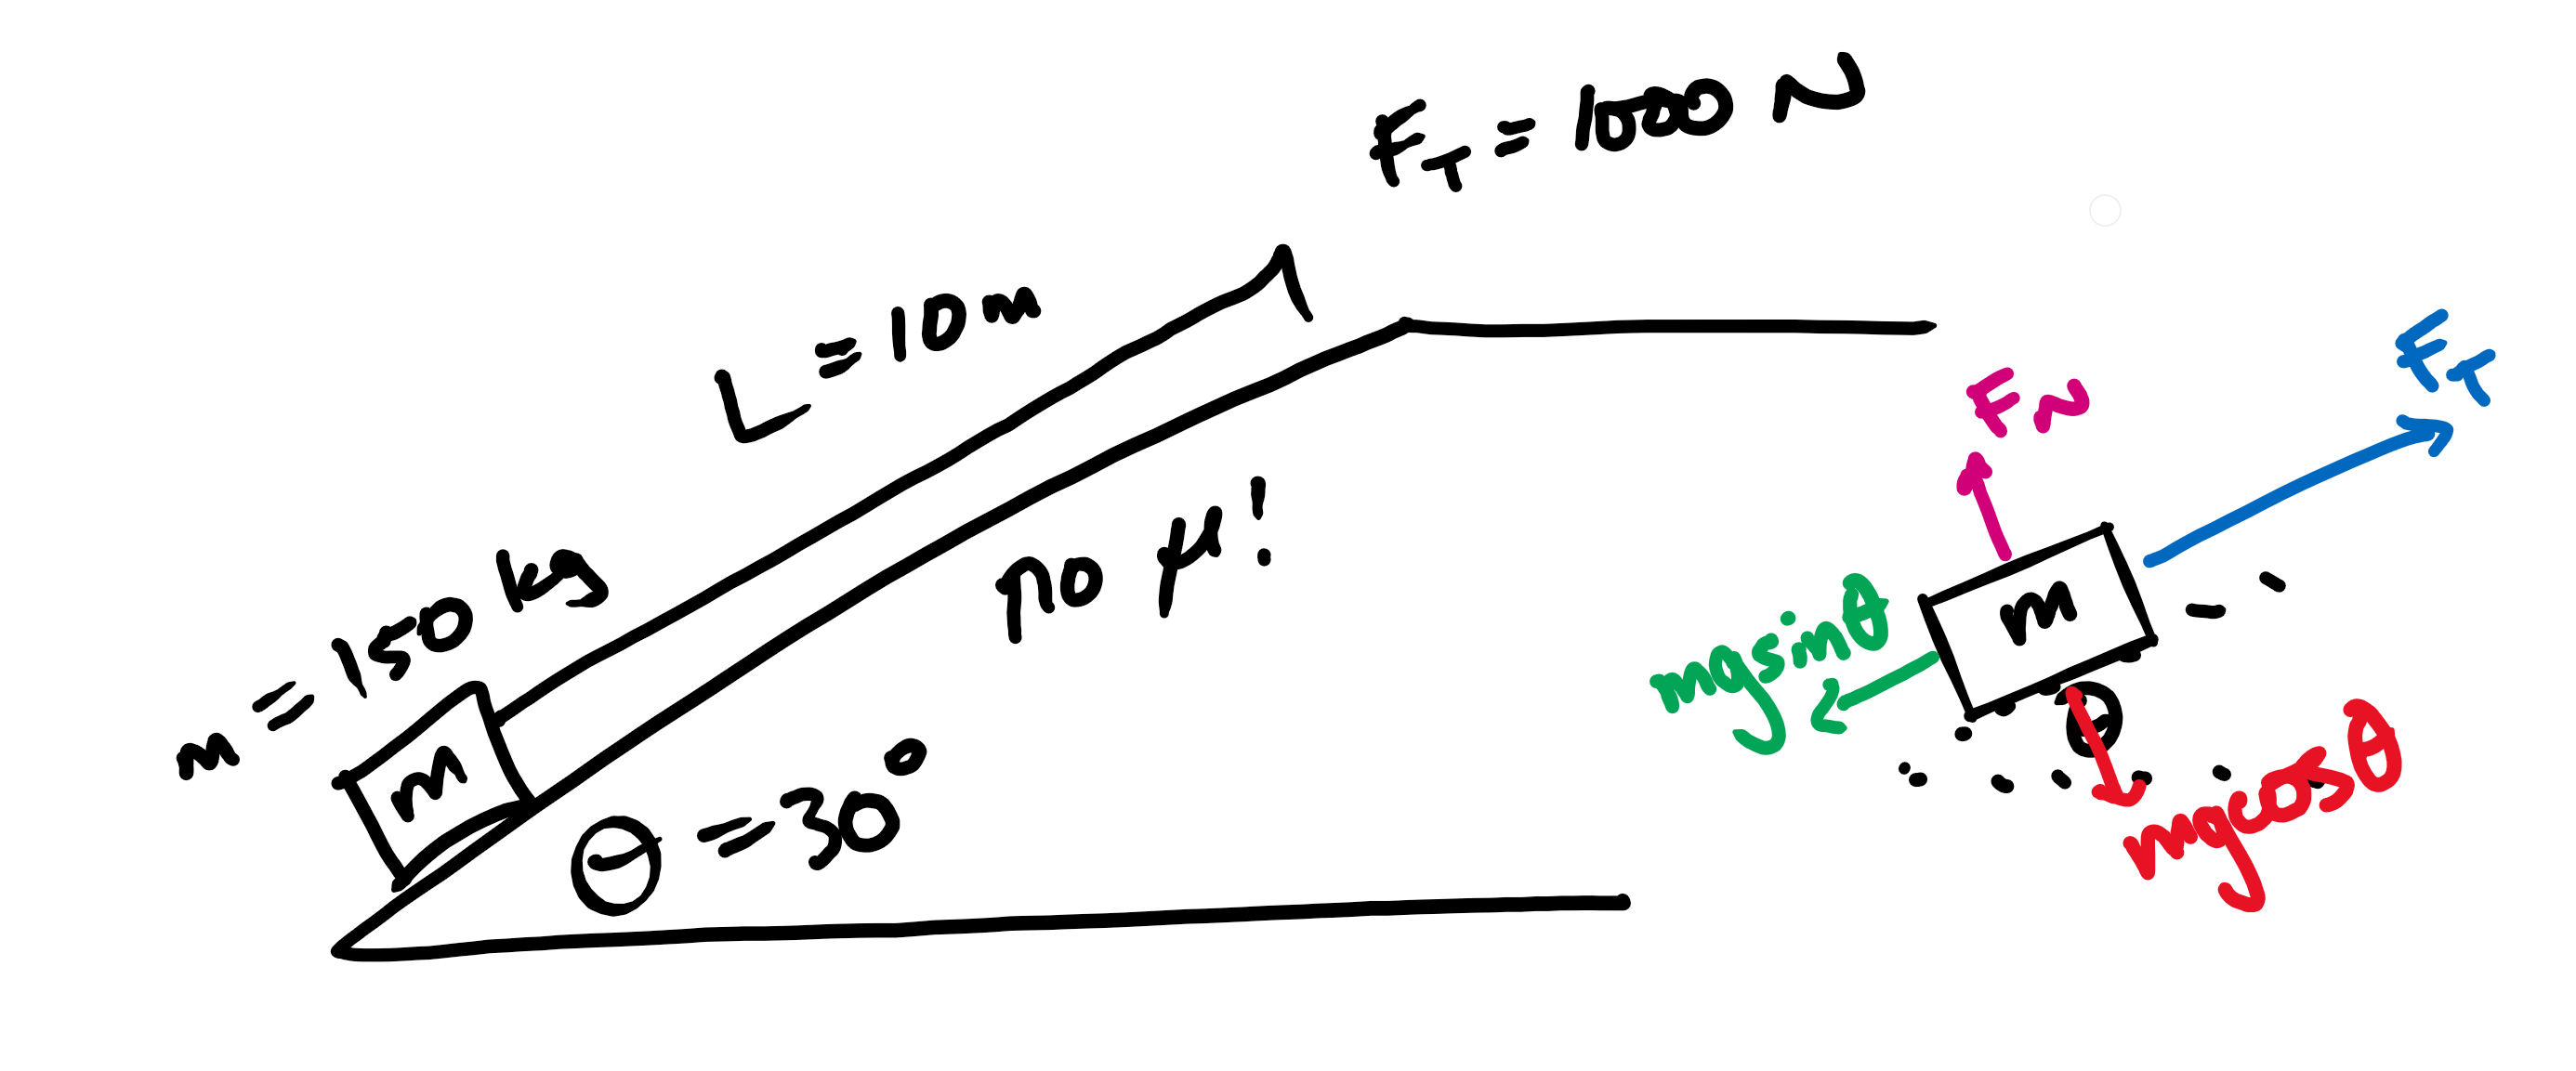
\includegraphics[width=0.5\textwidth]{chapters/ch4/images/fig4_5.PNG}
    \end{center}

    While this problem could be solved using kinematics and Newton's second law, we can also use the Work-Energy theorem. 

    $$
    \begin{aligned}
        W_{in} &= \Delta KE + \Delta PE\\
        F_T \cdot L &= \frac{1}{2}m(v_f - v_i)^2 + mg(h_f - h_i)\\
        F_T \cdot L &= \frac{1}{2}mv_f^2 + mgh_f\\
        v_f &= \sqrt{\frac{2(F_TL - mgh_f)}{m}}\\
        v_f &= \sqrt{\frac{2(F_TL - mg(L\sin\theta))}{m}}
    \end{aligned}
    $$
\end{problem}

\begin{problem}
    A skiier starts at the top of a mountain and is attached a spring at the bottom of the cliff. The skiier will also experience friction for 15m at the bottom of the slope right before the spring. How far was the spring compressed when the skiier reaches the bottom of the slope?

    \begin{center}
        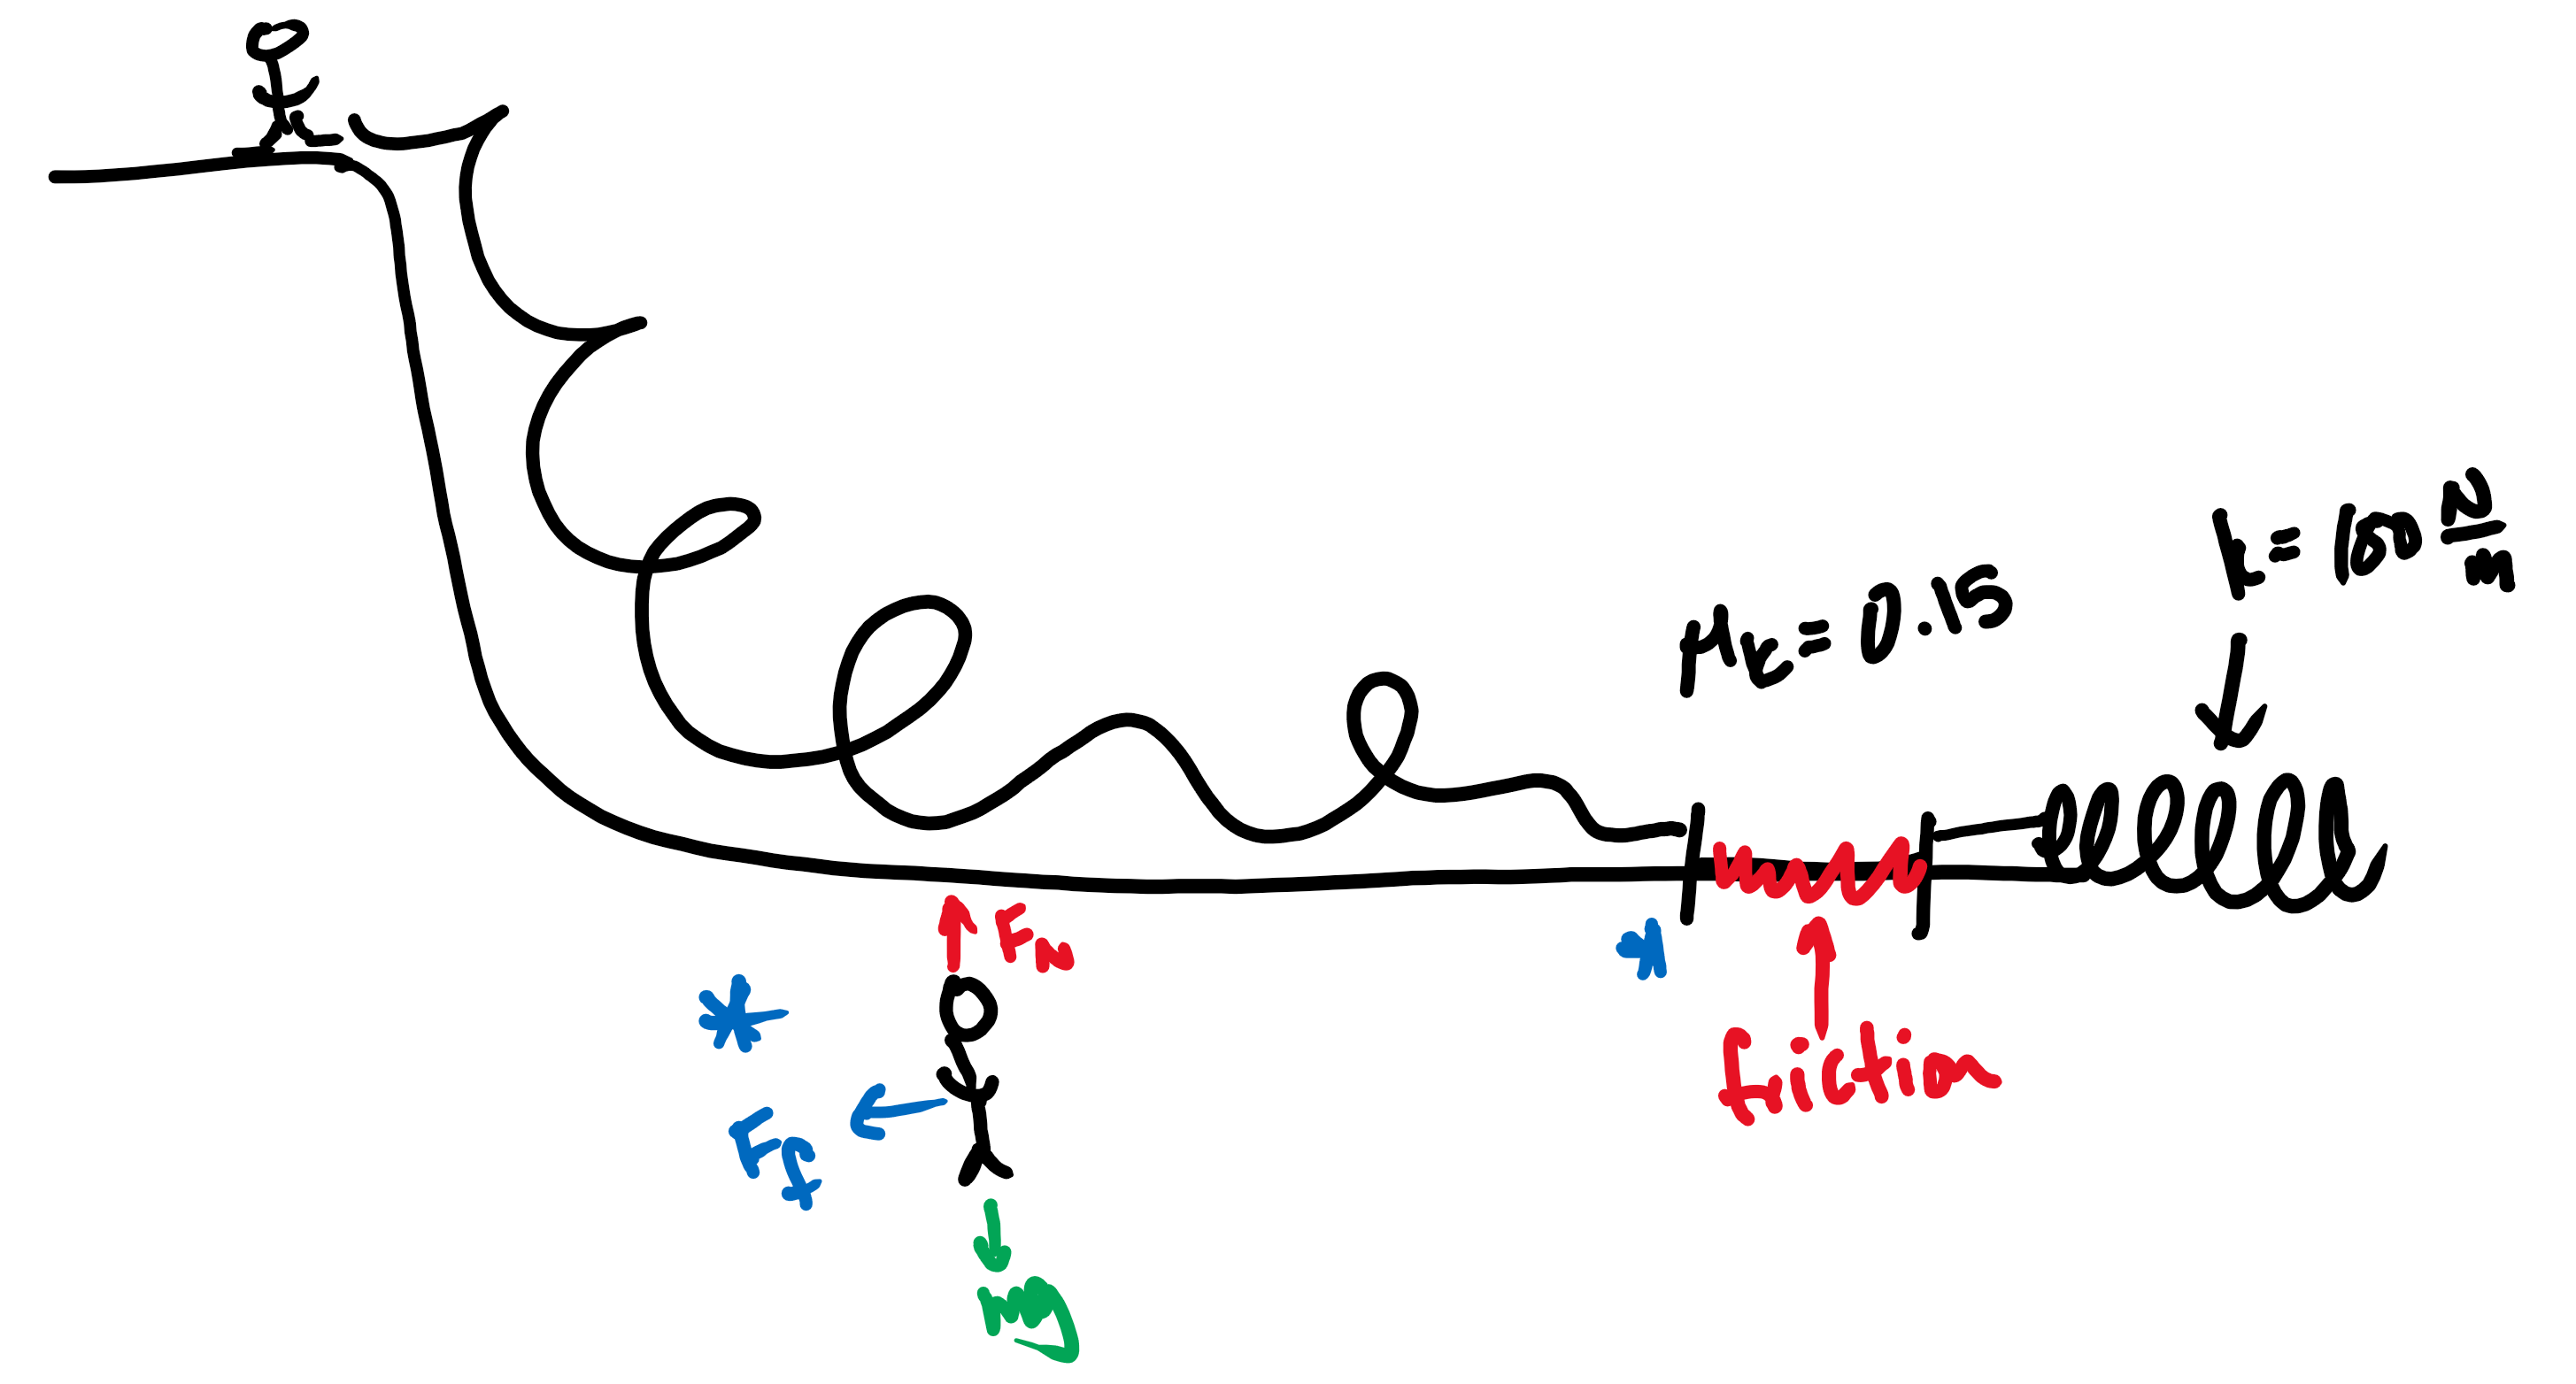
\includegraphics[width=0.5\textwidth]{chapters/ch4/images/fig4_6.PNG}
    \end{center}

    $$
    \begin{aligned}
        W_{in} = 0 &= \Delta PE + \Delta E_s + \Delta E_{T}\\
        0 &= mg(h_f-h_i) + \frac{1}{2}k(x_f-x_i)^2 + \mu_kmgD\\
        0 &= -mgh_i + \frac{1}{2}kx_f^2 + \mu_kmgD\\
        x_f &= \sqrt{\frac{(mgh_i-\mu_kmgD)^2}{k}}\\
        x_f &= \sqrt{\frac{((70\kg)(9.81\frac{\m}{\s^2})(50\m)-(0.15)(70\kg)(9.81\frac{\m}{\s^2})(15\m))^2}{150 \frac{\N}{\m}}}\\
    \end{aligned}
    $$
\end{problem}


\begin{problem}
    A stunt artist was launched out of a cannon on a 20m pedestal. He will land in a bucket attached to a pulley. The pulley also has a 50kg mass attached to it, and the bucket is 10m above the ground. Assume the bucket has no mass and the pulley exerts no friction on the string wrapped around the pulley. What is the speed of the stunt artist right when he lands in the bucket? 
    
    \begin{center}
        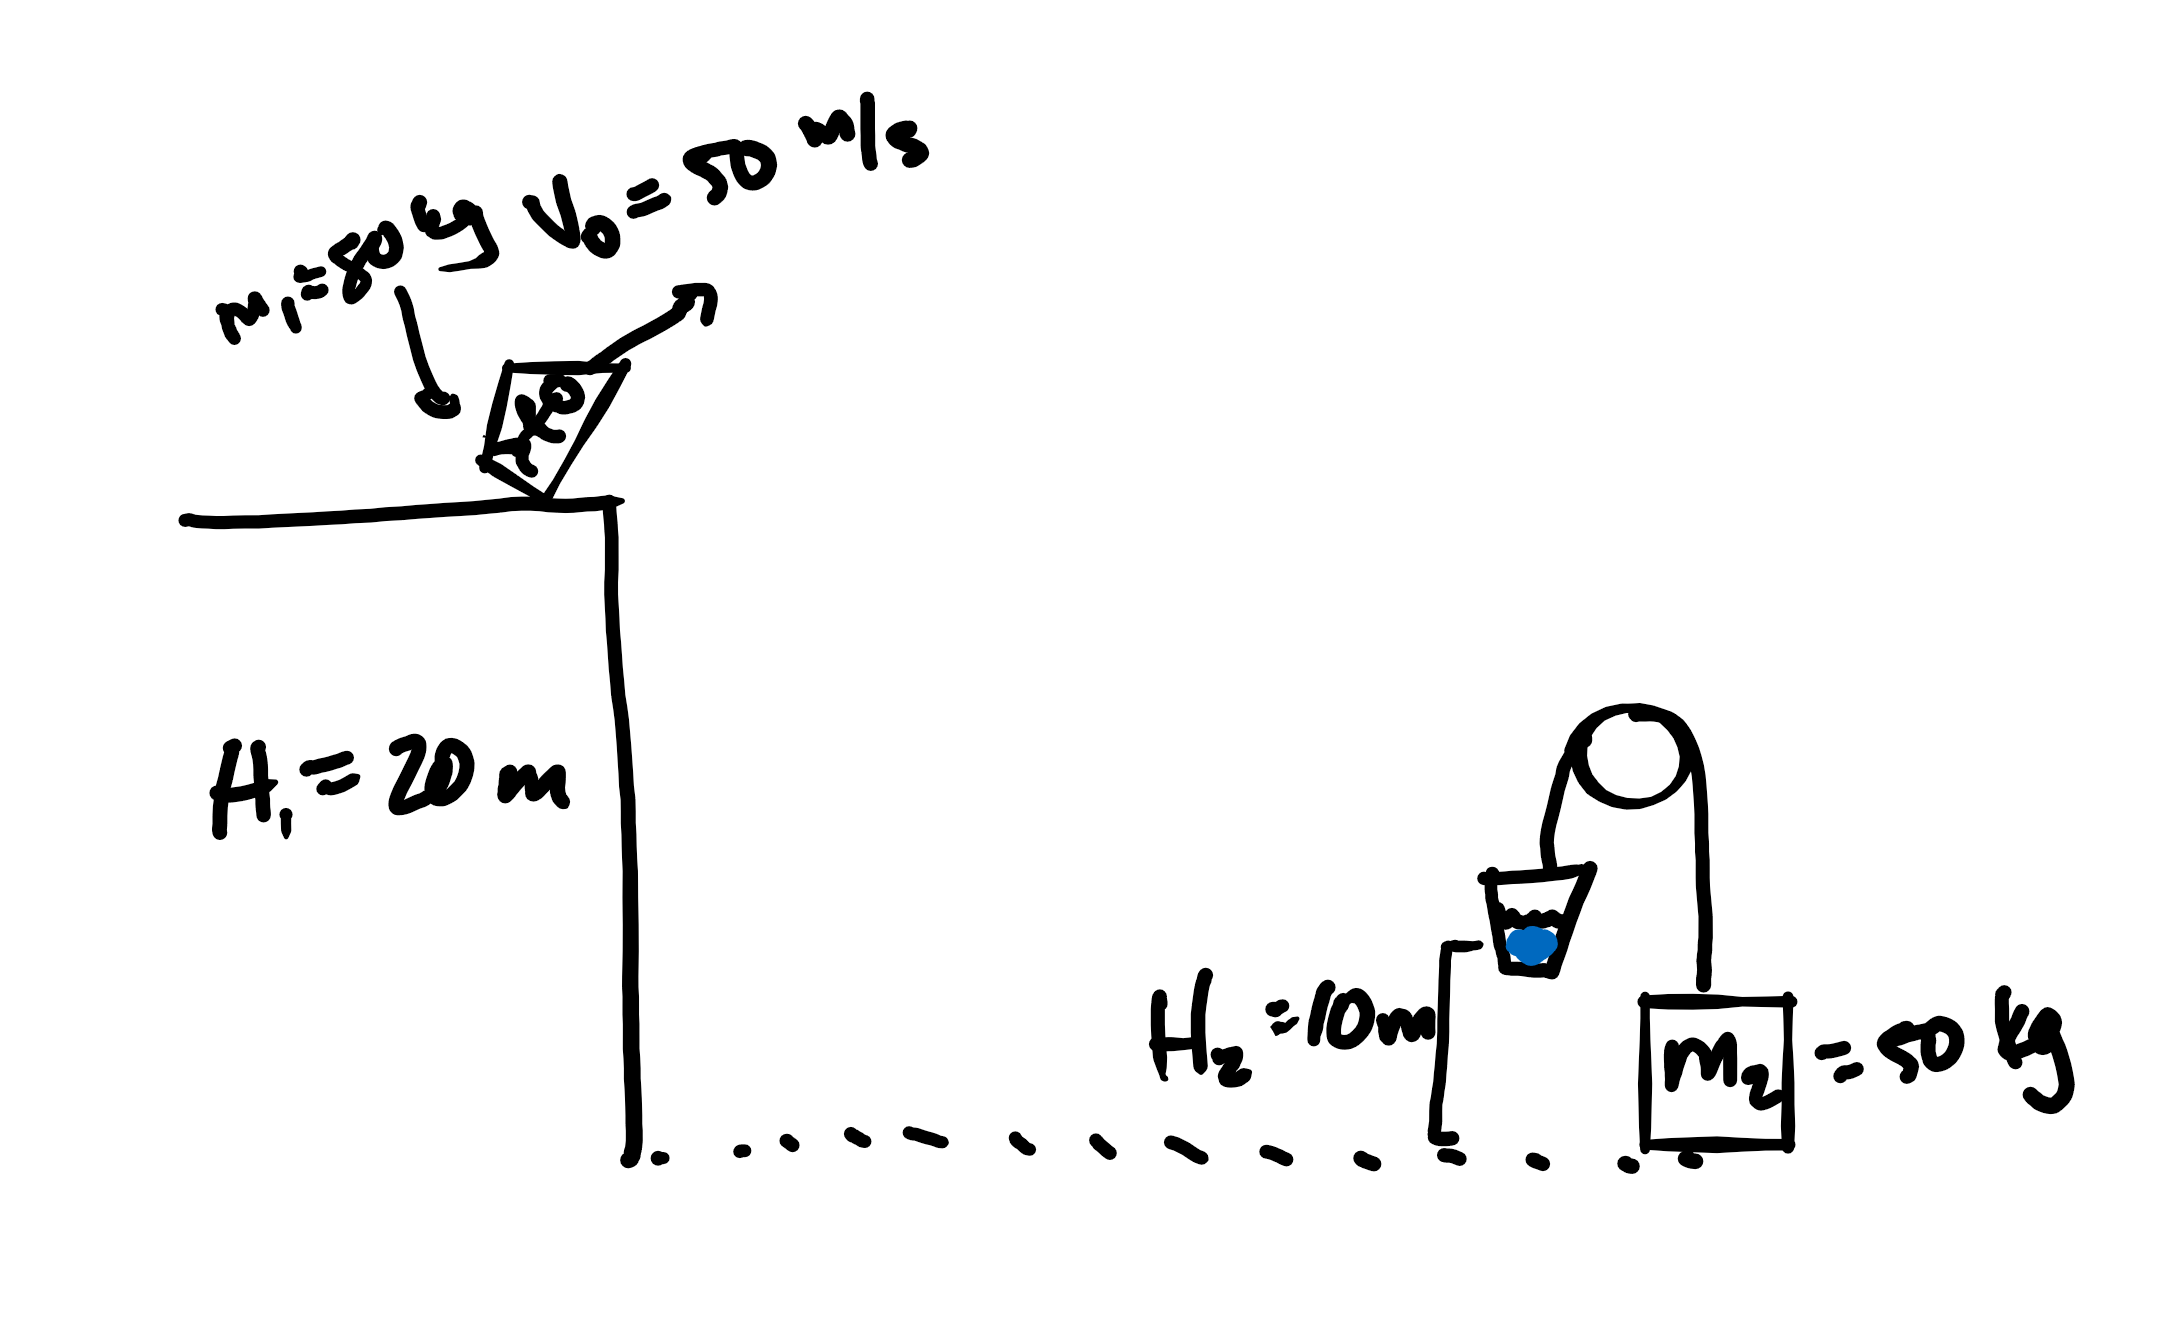
\includegraphics[width=0.5\textwidth]{chapters/ch4/images/fig4_7.PNG}
    \end{center}

    $$
    \begin{aligned}
        W = 0 &= \Delta KE_1 + \Delta PE_1 + \Delta KE_2 + \Delta PE_2\\
        0 &= \frac{1}{2}m(v_{f1}-v_{i1})^2 + \frac{1}{2}m_2(v_{f2}-v_{i2})^2 + m_1g(H_{f1} - H_{i1}) + m_2g(H_{f2} - H_{i2})\\
    \end{aligned}
    $$

    ANSWER: $41.3 \frac{\m}{\s}$
\end{problem}


\section{Work and Calculus}

\begin{itemize}
    \item Sometimes, the force being applied to an object over a given distance is variable
    \item If you are given an equation for what the force is (dependent on distance), then $W = \int_{x_i}^{x_f} F(x) dx$
\end{itemize}


\begin{problem}
    If the force applied to an object (as a function of distance) is $F(x) = 5 - 2x$, what is the work done on the object if the object moves 3 \m?

    $$
    \begin{aligned}
        W &= \int_{x_i}^{x_f} F(x) \: dx\\
        W &= \int_{0}^{3} 5-2x \: dx\\
        W &= (5-2(3))-(5-2(0)) = -1-5
        W &= -6 \J
    \end{aligned}
    $$
\end{problem}


\section{Power}

\begin{definition}[Power]{def4.5:label}
    \textbf{Power:} How much energy is expended over a given time interval.

    $$
    P = \frac{\Delta E}{\Delta t} = \frac{W}{t}
    $$

    \textbf{SI Units:} Watts (W)
\end{definition}


\begin{problem}
    A block of mass 1000 kg is attached to a pulley at the top of a building. The pulley is attached to a motor that uses 200 kW. What is the final velocity of the block the moment it reaches the top of the building?

    \begin{center}
        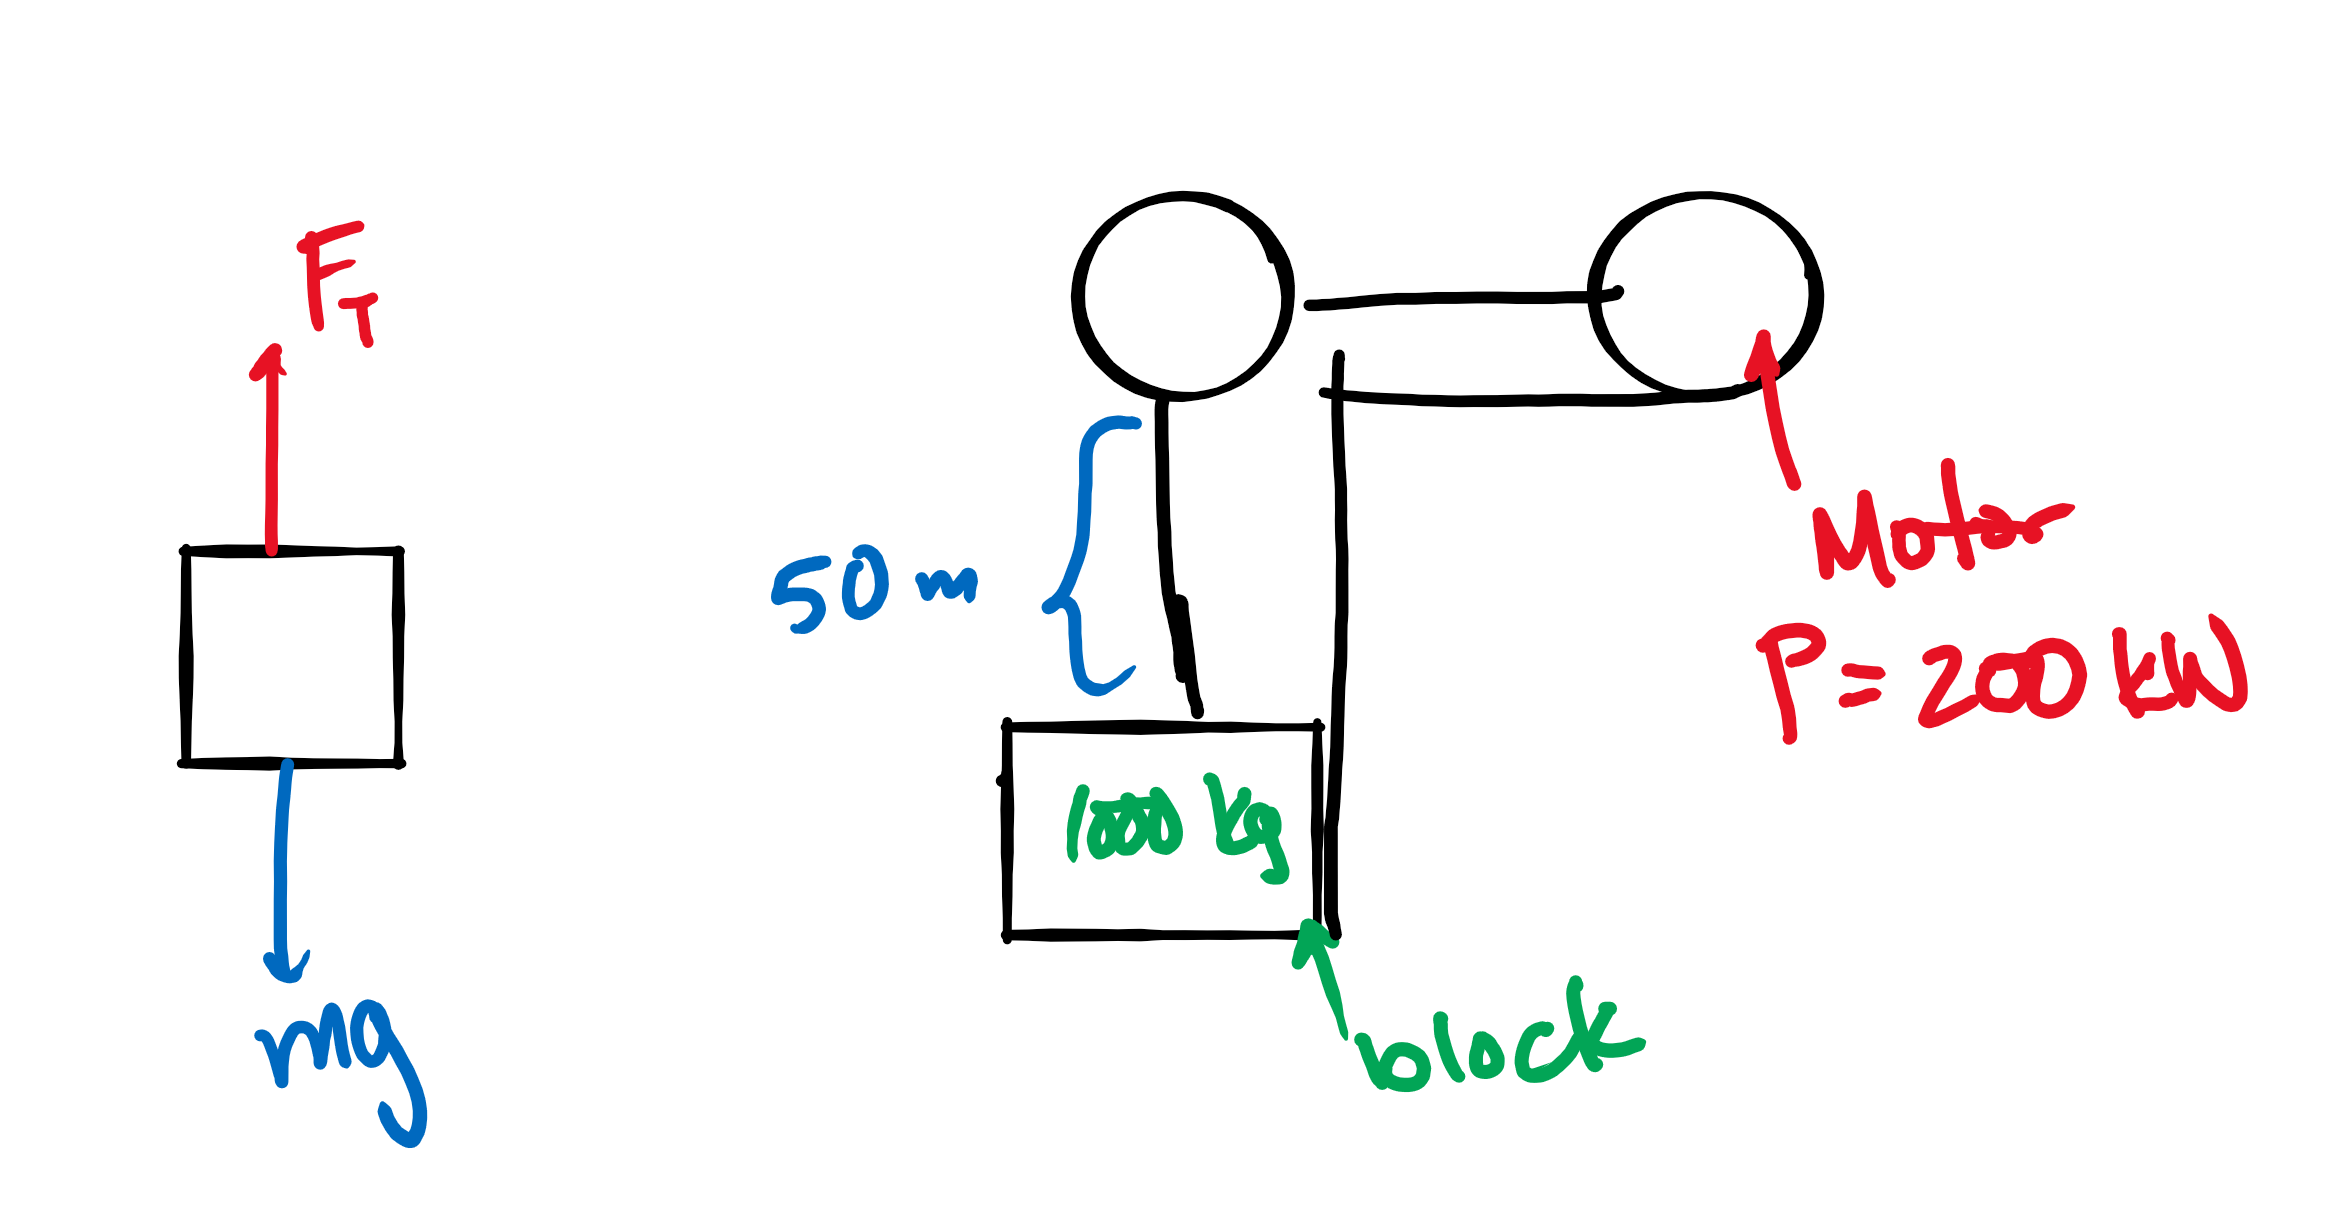
\includegraphics[width=0.5\textwidth]{chapters/ch4/images/fig4_8}
    \end{center}

    $$
    \begin{aligned}
        P &= \frac{\Delta E}{\Delta t}\\
        P &= \frac{\Delta KE + \Delta PE}{\Delta t}\\
        P &= \frac{\frac{1}{2}mv^2+mgh}{\Delta t}\\
        v_f &= \sqrt{\frac{2(-mgh+\Delta T P)}{m}}
    \end{aligned}
    $$
\end{problem}


\begin{problem}
    A truck drives up a ramp with an angle of inclination of $15^\circ$. If the truck drives 200 meters in 20 seconds, what is the power of the truck (in kW) after the truck has moved 200 meters? Assume that 10\% of the total energy is lost to the environment.

    $$
    \begin{aligned}
        P &= \frac{\Delta E}{t}\\
        P &= \frac{\Delta KE + \Delta PE}{t}+ 10\%\text{ energy}\\
        P &= \frac{\frac{1}{2}mv^2 + mgh}{t} + 10\%\text{ energy}\\
        P &= \left[\frac{\frac{1}{2}m\left(\frac{\Delta x}{t}\right)^2 + mgL\sin\theta}{t}\right]\frac{1}{0.9}\\
        P &= 98.3 \text{ kW}
    \end{aligned}
    $$
\end{problem}


\chapter{Counting}


\chapter{Advanced Counting}



\chapter{Relations}


\chapter{Graphs}



\chapter{Trees}

\end{document}
